\section{Related Work}\label{sec:relatedwork}
This chapter sums up all the related work that has been done on bx. Section \ref{subsec:existingdemo}, \ref{subsec:virtualmachines}, \ref{subsec:handbook}, and \ref{subsec:examplerep} describe the various ways that bx community and developer's group have tried to make the work done on bx visible to the world. Finally, Section \ref{subsec:discussion} explains the related problems and their comparison with my demonstrator i.e., Demon-BX. 

Model transformation is a central part of Model-Driven Software Development \cite{bx-grace} \cite{bx-dagstuhl}. Bx community has been constantly doing research and development work in many fields to help people understand and increase awareness about bx. Nowadays, researchers from different areas are actively investigating the use of bx to solve a variety of problems. A lot of work has been done in terms of building usable tools and languages for bx. These tools can be used in various fields, for achieving \textit{bidirectional transformation}. To understand these tools, several handbooks, tutorials and examples have been created so that users and developers can understand the core concepts. Following sections will describe these concepts in detail.

\subsection{Existing Demonstrator}\label{subsec:existingdemo}
First, I analyzed an existing demonstrator available along with the test cases of a domain-specific language, BiYacc \cite{biyacc} which is based on BiGUL \cite{bigul}. BiYacc designed to keep the parsers and printers needed by the language designers unified, in a single program, and consistent throughout the evolution of a language. Based on bidirectional transformations theory, BiYacc constructs the pairs of parsers and reflective printers and guarantees that they are consistent.

\begin{figure}
	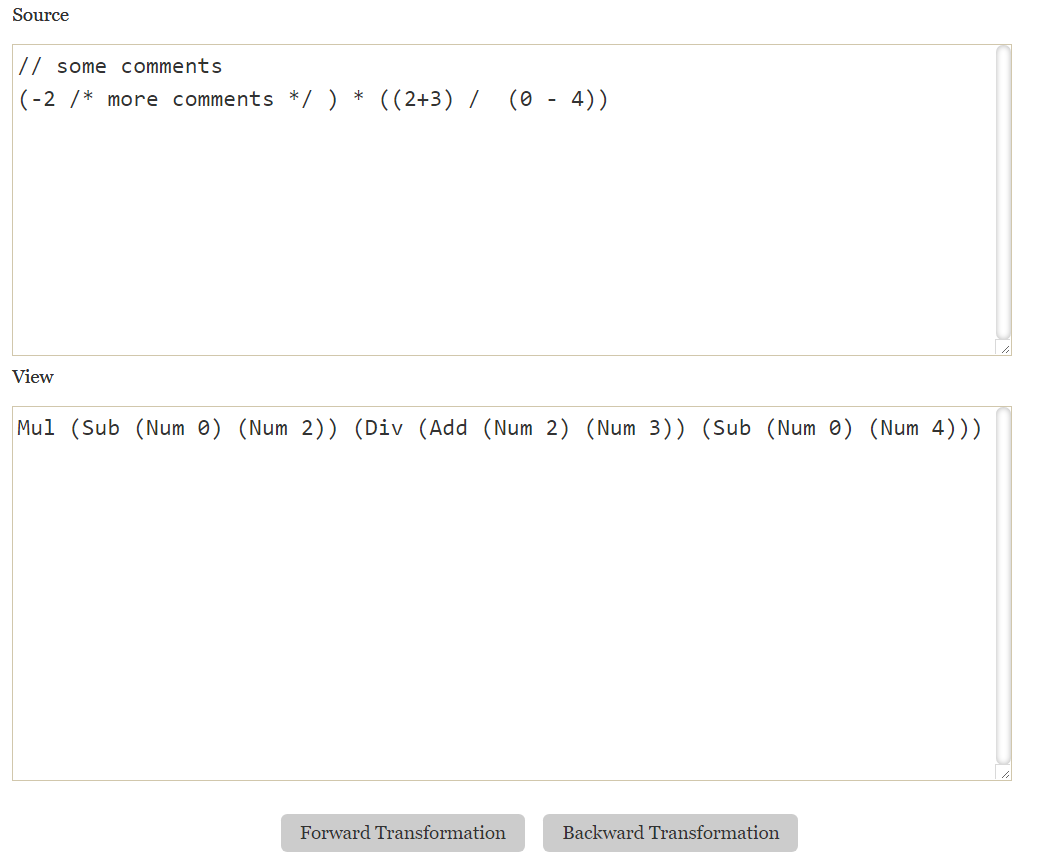
\includegraphics[width=1\textwidth]{figures/Biyacc}
	\caption{Web GUI for Demonstrator: Biyacc}
	\label{fig:WebGUI_Biyacc}
\end{figure}

Figure~\ref{fig:WebGUI_Biyacc} shows the web interface of the demonstrator. It contains two views i.e, source and view. Depending on the user selection, "source" contains an arithmetic expression or a program with some comments. After the forward transformation is done, "view" is loaded with the parsed version (machine readable format) of the sources' text.\\  
Being an online demonstrator, a user can try it out instantly and check how it works. It doesn't require any installation or technical expertise to get the example running.

\subsection{Virtual Machines}\label{subsec:virtualmachines}
Secondly, I have analyzed a web-based virtual machine, e.g., SHARE~\cite{share}. Basically, this is a web portal used for creating and sharing executable research papers and acts as a demonstrator to provide access to tools, software, operating systems, etc., which are otherwise a headache to install \cite{share}. Also, I have analyzed VM Virtual Box~\cite{virtualbox}, an open source virtualization product used for creating and sharing enterprise, academic, and personal work. Bx community has prepared a collection of virtual machines (e.g., for various TGG tools) hosted on SHARE and VM Virtual Box.

These virtual machines provide the environment that the user requires to execute his/her tool or program. Hence, it reduces the overhead of a user for maintaining and organizing all software framework related stuff and simplifies the access process for end-users. To access the shared material, virtual machine either have to accessed online or deployed on users' machine.

\subsection{Handbooks \& Tutorials}\label{subsec:handbook}
As a part of my research, I also analyzed some tutorials and tools and below are my findings.

Anjorin et al.~\cite{emoflon-part4} present the concept for \textit{bidirectional transformation} using Triple Graph Grammars (denoted by "TGG")~\cite{tgg}. To demonstrate their core idea and the usage of the tool, they have described an example by transforming one model (source) into another (target) through TGG transformations \cite{tgg}\cite{bx-tgg}. The whole tutorial is about 42 pages long which guides the user to get the example running through a series of steps. These steps include installing \ac{Eclipse}, getting their tool as an Eclipse plugin, setting up the workspace, creating TGG schema and specifying its rule and much more. If the user is able to execute each step correctly, then finally he/she can view the final output. It took me 4 days to get the tool up and running.

I have analyzed a tutorial\cite{bigul-tutorial} on a bidirectional programming language BiGUL\cite{bigul}. The core idea with BiGUL is to write only one putback transformation, from which the unique corresponding forward transformation is derived for free. The whole tutorial is about 45 pages long which includes a lot of complex formulas, algorithms, and guides the user to get the example running through a series of steps. These steps include installing BiGUL, setting up the environment, achieving bx through BiGUL's bidirectional programming and much more. If the user is able to execute each step correctly, then finally he/she can view the final output. 

\subsection{Example Repositories}\label{subsec:examplerep}
A rich set of bx examples repository \cite{bx-examples} has been created based on many research papers. These examples cover a diverse set of areas such as business process management, software modeling, data structures, database, mathematics and much more.

\begin{figure}
	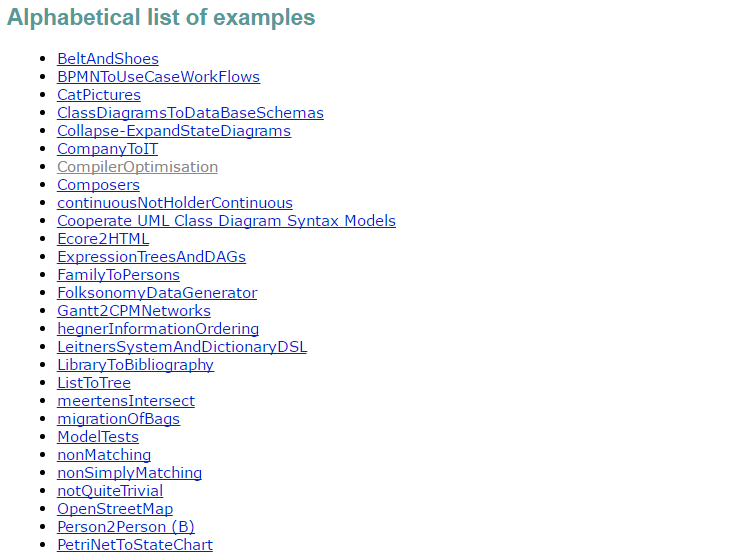
\includegraphics[width=0.7\textwidth]{figures/Bx_ExampleRepo}
	\caption{BX Example Repositories}
	\label{fig:Bx_ExampleRepo}
\end{figure}

Figure~\ref{fig:Bx_ExampleRepo} shows a screenshot of the example repositories listed alphabetically on the bx community web-site (\url{http://bx-community.wikidot.com/}). A user can find relevant information about the examples on the respective web pages. Some of the examples are very well documented along with class diagrams, activity diagrams, object diagrams etc. and source code of a few examples are available as well.

\subsection{Discussion}\label{subsec:discussion}
In this section, I will discuss the related problems associated with each of the related work discussed in the previous sections and a comparison of these related work with the Demon-BX tool.

\subsubsection{Related Problems}\label{subsubsec:relatedproblems}
Associated problems that I found with the above discussed related work are described in the following paragraphs: 

\paragraph{Existing Demonstrator}
The existing demonstrator's visual representation doesn't create interest in the target audience as it does not exploit the potential of using an interactive GUI and colors, etc. It just makes use of two text fields and is comparable to a console-based interface that is accessible online.

There is very limited guidance provided concerning what the user can do and try out with the demonstrator. Especially for non-experts, it is not clear what to do with the demonstrator after a few minutes.

The existing demonstrator is based on a rather technical example that might not be relevant, interesting, or convincing for a large group of potential bx users.

\paragraph{Virtual Machines}
For security reasons, web-based virtual machine, e.g., SHARE is not like other web portals where a user need to simply sign-up and can host/create/access data, rather it includes a series of request-grant cycle for getting access to an environment and hosting/managing data. Also, some actions require special authorization and take time to complete the whole process.

The user needs at least 3 Gigabyte or more space on his/her local system for configuring the virtual machine i.e., VM Virtual Box depending on the requirement of the environment, which sometimes creates an overhead.

\paragraph{Handbooks \& Tutorials}
As described in handbooks and tutorials, installation process is time consuming and requires technical expertise as the user typically has to setup and install the tool. Required knowledge is too tool/area specific and it can be challenging if the user is not familiar with the technological space, e.g., the user must possess knowledge about Java and Eclipse framework or a Java programmer might find the tool chain for Haskell unfamiliar.

Steps to get the example running needed technical expertise, e.g., In some cases, domain-specific knowledge includes mathematics and specific coding language. What is showcased and discussed is tied to a specific technological space and might not be easily transferable to other bx approaches and also, not very helpful to understand what bx is before deciding which bx tool to use.

\paragraph{Example Repositories}
In today's fast paced and visually enriched world, "what you see is what you believe" and that
is exactly what these examples are lacking in. None of the examples have a demonstrator
showing how it works. Hence, it is very difficult for a user to realize the examples just by going
through the documentation and UML diagrams. Even if the source code is present, it takes a lot
of time and requires technical expertise to set-up the framework and get the example running.

\subsubsection{Comparison}\label{subsubsubsec:comparison}
Associated problems as discussed in Section \ref{subsubsec:relatedproblems} gave me the foundation while forming the requirements for my demonstrator. To overcome these problems, I took the shortcomings from each related work and designed the functional and non-functional requirements. 

Based on the requirements described in chapter \ref{sec:requirements} and considering the problems as discussed in Section \ref{subsubsec:relatedproblems}, Table~\ref{tab:comparison_relatedwork} illustrates a comparison between all the related work discussed above with the Demon-BX tool. "\checkmark" denotes the fulfillment of the requirement, "\ding{55}" denotes the non-fulfillment of the requirement, and "?" denotes insufficient information about the requirement. This comparison table clearly shows that Demon-BX tool overcomes all the problems associated with these related work.

\begin{sidewaystable}
	\centering
	\begin{tabular}{|lcccccccccccccc|}
		\hline
		\textbf{} & \multicolumn{14}{c|}{\textbf{Requirements}} \\
		\textbf{Related Work} & \textbf{FR1} & \textbf{FR2} & \textbf{FR3} & \textbf{FR4} & \textbf{NR1} & \textbf{NR2} & \textbf{NR3} & \textbf{NR4} & \textbf{NR5} & \textbf{NR6} & \textbf{NR7} & \textbf{NR8} & \textbf{NR9} & \textbf{NR10} \\
		\hline
		\hline
		Existing Demon. & \ding{55} & \checkmark & \checkmark & \checkmark & \checkmark & \ding{55} & \ding{55} & \ding{55} & \ding{55} & \checkmark & \checkmark & \checkmark & \checkmark & ? \\ 
		\hline
	    Virtual Machines & \checkmark & \checkmark & \ding{55} & \ding{55} & \ding{55} & \checkmark & \checkmark & \ding{55} & \ding{55} & \checkmark & \ding{55} & \ding{55} & \checkmark & \ding{55} \\
	    \hline
		Handbooks \& Tutorials & \checkmark & \checkmark & \ding{55} & \ding{55} & \ding{55} & \checkmark & \checkmark & \checkmark & \ding{55} & \checkmark & \ding{55} & \ding{55} & \ding{55} & \ding{55} \\
		\hline
		Example Repositories & \ding{55} & \ding{55} & \ding{55} & \ding{55} & \ding{55} & \ding{55} & \checkmark & \ding{55} & \checkmark & \checkmark & \checkmark & \checkmark & \ding{55} & \checkmark \\
		\hline
		Demon-BX & \checkmark &  \checkmark & \checkmark & \checkmark & \checkmark & \checkmark & \checkmark & \checkmark & \checkmark & \checkmark & \checkmark & \checkmark & \checkmark & \checkmark \\
		\hline
	\end{tabular}
	\caption{Comparison of related work and Demon-BX based on requirements}
	\label{tab:comparison_relatedwork}
\end{sidewaystable}